
\documentclass[xcolor=dvipsnames]{beamer} 
\usetheme{default} 

\usecolortheme[named=Blue]{structure}
\usetheme[height=7mm]{Rochester} 
\setbeamertemplate{items}[ball] 
\setbeamertemplate{blocks}[rounded]
\setbeamertemplate{navigation symbols}{} 

\usepackage{tikz} 
\usetikzlibrary{shapes.arrows,chains,positioning}

\begin{document}

% -------------------------------------------------------------------------
%
% -------------------------------------------------------------------------

\title{Embedded Languages for Data-Parallel Programming} 
\author[J. Svensson]{Bo Joel Svensson} 
\institute{ 
  Department of Computer Science and Engineering \\ 
  Chalmers University of Technology 
} 

% -------------------------------------------------------------------------
%
% -------------------------------------------------------------------------

\begin{frame}[plain] 
  \titlepage
\end{frame} 


\section{background} 

% -------------------------------------------------------------------------
%
% -------------------------------------------------------------------------
\begin{frame}{Data-Parallelism}
\begin{center} 
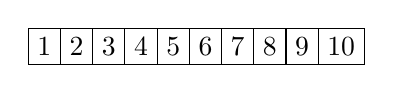
\begin{tikzpicture}[
      start chain=1 going right,start chain=2 going below,node distance=-0.15mm
    ]

  \foreach \x in {1,2,...,10} {
    \node (\x) [draw, on chain=1] {\x};
  }

\end{tikzpicture} 
\end{center}

%% \begin{block}{Code 1}
%% \begin{verbatim}
%% Hej
%% \end{verbatim} 
%% \end{block}

\end{frame}

% -------------------------------------------------------------------------
%
% -------------------------------------------------------------------------
\section{GPUs and CUDA}

\begin{frame}{GPU Programming}
\begin{center} 

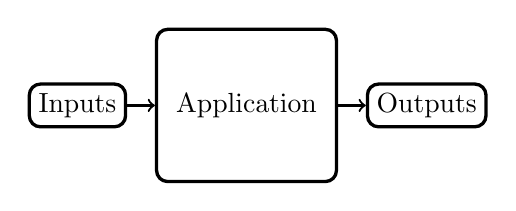
\begin{tikzpicture}[
      start chain=1 going right,start chain=2 going below,node distance=1em,
      every join/.style={->,thick},
    ]

  \node [draw,very thick, rounded corners, on chain=1,join] {Inputs}; 
  \node [draw,very thick, rounded corners, on chain=1,minimum height=5.5em,minimum width = 6.5em,join] {Application}; 
  \node [draw,very thick, rounded corners, on chain=1,join] {Outputs}; 
  

\end{tikzpicture} 
\end{center}

\end{frame}

% -------------------------------------------------------------------------
%
% -------------------------------------------------------------------------
\section{GPUs and CUDA}

\begin{frame}{GPU Programming}
\begin{center} 

\begin{tikzpicture}[remember picture,
      start chain=going right,
      outer/.style={on chain, node distance=1em},
      every join/.style={->,thick},
      inner/.style={circle,draw=blue!50,fill=blue!20,thick,inner sep=1pt},
    ]

  \node [outer,draw,very thick, rounded corners,join] {Inputs}; 
  \node [outer,draw=gray!50,very thick, rounded corners,minimum height=5.5em,minimum width = 6.5em,join] (apa) {
    \begin{tikzpicture} 
      \node [draw=black!100,inner,minimum size=1pt] (k1) {k1};
      \node [draw=black!100,inner,minimum size=1pt, below= 1em of k1] (k2) {k2};
      \node [draw=black!100,inner,minimum size=1pt, right= 1em of k1] (k3) {k3}; 
    \end{tikzpicture}

  }; 
  \node [outer,draw,very thick, rounded corners,join] {Outputs}; 
  

  \draw (k1) -> (k3);
  \draw (k2) -> (k3); 
  \draw (apa.west) -> (k1.west); 
  \draw (apa.west) -> (k2.west); 
  \draw (k3.east) -> (apa.east); 
  

\end{tikzpicture} 
\end{center}

\end{frame}


% -------------------------------------------------------------------------
%
% -------------------------------------------------------------------------
\section{Embedded Languages}

% -------------------------------------------------------------------------
%
% -------------------------------------------------------------------------
\section{Obsidian}

% -------------------------------------------------------------------------
%
% -------------------------------------------------------------------------
\section{EmbArBB} 

% -------------------------------------------------------------------------
%
% -------------------------------------------------------------------------
\section{Future Work}


\end{document} 
